% !TEX root = Séquence 2 - Activités - Vecteurs.tex
% Transcription de l'activité 3 (Enchaîner deux translations) du manuel,
% en autonome (même montage que "Séquence 2 - Cours - Vecteurs.tex" : on
% recharge CLT2627.sty par \input direct à cause de l'espace dans le nom
% du dossier).
\documentclass[a4paper,11pt,french]{report}
\input{../TeX - Polycopié et Exercices/CLT2627.sty}
\graphicspath{{../TeX - Polycopié et Exercices/}}

\usetikzlibrary{shapes.misc, arrows.meta}
\tikzset{cross/.style={cross out, draw=black, minimum size=#1, inner sep=0pt}}

\begin{document}
\pagestyle{empty}
\fancypagestyle{plain}{\fancyhf{}\renewcommand{\headrulewidth}{0pt}\renewcommand{\footrulewidth}{0pt}}

% ----------------------------------------------------------------------
% Titre de séquence, repris tel quel de "Séquence 2 - Cours - Vecteurs.tex"
% (coins arrondis, étiquette posée via overlay qui entaille le cadre en
% haut à gauche, grand titre centré en dessous), pour un rendu cohérent
% avec le cours et la feuille d'exercices. #1 = largeur (fraction de
% \linewidth), #2 = étiquette, #3 = titre.
% ----------------------------------------------------------------------
\newcommand{\SequenceTitre}[3]{%
  \begin{center}
  \begin{tcolorbox}[
    enhanced,
    width=#1\linewidth,
    colback=white,
    colframe=black,
    boxrule=0.8pt,
    arc=8pt,
    sharp corners=downhill,
    left=10pt, right=10pt, top=8pt, bottom=6pt,
    halign=center,
    overlay={
      \node[fill=white, anchor=west, font=\normalsize, inner xsep=4pt]
        at ([xshift=14pt]frame.north west) {#2};
    },
  ]
  {\huge #3}
  \end{tcolorbox}
  \end{center}
}

\newtcolorbox{JauneBox}{enhanced,colback=yellow!12,colframe=yellow!55!black,
  boxrule=0.6pt,arc=2pt,left=6pt,right=6pt,top=4pt,bottom=4pt}

% Point représentant le palet : petit cercle avec une croix à l'intérieur.
\newcommand{\Palet}[1]{\node[draw,circle,inner sep=1.3pt] at #1 {\tiny$+$};}

\SequenceTitre{0.78}{Séquence 2}{Découverte de la somme}
\vspace{4pt}

On s'intéresse au mouvement subi par le palet au cours d'un jeu de hockey sur glace, la patinoire étant vue de dessus. Tout part de la crosse d'Alfred (le point $A$) : le palet va maintenant voyager de joueur en joueur au fil de plusieurs passes, chaque passe correspondant à... une translation !

\begin{enumerate}
\item
\begin{enumerate}
\item Alfred fait une passe à Benoît en suivant la translation de vecteur $\Vj{u}$ : placer le point $B$ qui correspond à l'emplacement de Benoît.
\item Sans perdre une seconde, Benoît relance vers Camille avec la translation de vecteur $\Vj{w}$ : placer le point $C$.
\item Deux passes, mais un seul déplacement final : le palet a subi le même déplacement qu'avec une seule et longue passe directe d'Alfred à Camille. Tracer le vecteur qui correspond à cette passe unique.
\end{enumerate}
\end{enumerate}

\begin{center}
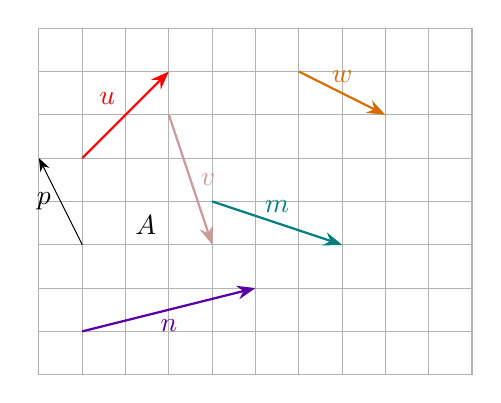
\begin{tikzpicture}[scale=0.55, >=Stealth]
\draw[thin,gray!60] (0,0) grid (10,8);
\Palet{(2,3)} \node[above right] at (2,3) {$A$};

\draw[->,thick,red] (1,5) -- (3,7) node[midway,above left]{$\Vj u$};
\draw[->,thick,orange!85!black] (6,7) -- (8,6) node[midway,above]{$\Vj w$};
\draw[->,thick,violet!70!blue] (1,1) -- (5,2) node[midway,below]{$\Vj n$};
\draw[->,thick,teal] (4,4) -- (7,3) node[midway,above]{$\Vj m$};
\draw[->,thick,pink!80!black] (3,6) -- (4,3) node[midway,right]{$\Vj v$};
\draw[->,thin,black] (1,3) -- (0,5) node[midway,left]{$\Vj p$};
\end{tikzpicture}
\end{center}

\begin{JauneBox}
L'enchaînement de ces deux translations correspond à la translation de vecteur $\Vj u+\Vj w$.
\end{JauneBox}

\begin{enumerate}
\setcounter{enumi}{3}
\item[d)] Il y a un autre représentant de ce vecteur dans ceux déjà tracés sur le schéma\dots{} Lequel ?\\
\textcolor{white}{Le vecteur $\Vj u+\Vj w$ est égal au vecteur $\Vj n$ de la figure.}
\end{enumerate}

\begin{enumerate}
\setcounter{enumi}{1}
\item
\begin{enumerate}
\item Le match continue : Camille relance vers David selon la translation de vecteur $\Vj p$. Sans perdre de temps, David envoie à Éric selon la translation de vecteur $\Vj v$. Placer le point $E$ représentant la position d'Éric.
\item Comme avant, représenter un vecteur qui correspond à ce double relais, c'est-à-dire à $\Vj p+\Vj v$.
\end{enumerate}
\end{enumerate}

\end{document}
